\documentclass[pdf]{beamer}
%\documentclass[notes]{beamer}
%\documentclass{beamer}
\usepackage[utf8]{inputenc}
\usepackage{lmodern}
\usepackage{colortbl}

%\usepackage{scrextend}
%\changefontsizes{7.5pt}


\makeatletter
\makeatother
\usepackage{graphicx}

\mode<presentation>{\usetheme{Warsaw}}
%\mode<presentation>{\usetheme{Madrid}}
%% preamble
\title{Métodos multivariados de Análisis de Datos}
\subtitle{Análisis de nutrientes en pizzas}

\author{
Ricardo Cruz Sánchez \\
  \and
Rolando Corona Jiménez
}

\institute[CIMAT]{CIMAT}


\begin{document}

\begin{frame}
\titlepage
\end{frame}

%\AtBeginSubsection[]
%{
%  \begin{frame}<beamer>
%    \frametitle{Contenido}
%    \tableofcontents[currentsection,currentsubsection]
%  \end{frame}
%}

\section{Resumen}

\begin{frame}{Resumen}
\begin{enumerate}
\item primeros lugares en morbilidad y mortalidad a nivel mundial.
\item la hiperglucemia causa alteraciones en el metabolismo de la glucosa y l\'ipidos.
\item El padecimiento es cr\'onico-degenerativo
\item Desde el a\~no 2000, la diabetes mellitus en M\'exico es la primera causa de muerte entre las mujeres y la segunda entre los hombres
\item la edad, la obesidad, el sedentarismo, la alimentación inadecuada, los antecedentes familiares y algunos factores gen\'eticos
\item detección temprana
\item Incorporación de base de conocimiento en RB.
\end{enumerate}
\end{frame}


\section{Estado de investigación}
\begin{frame}{Estado de investigación}
El proyecto fue inspirado en el trabajo de Jeroen Eggermont y Joost N. Kok, quienes en su paper \underline{\textit{Genetic Programming for data classification: partitioning the search space}} exploran modelos para la clasificaci\'on de pacientes de nacionalidad americana con presencia o ausencia de DM2.\\

Los modelos presentados sugieren la posibilidad de extrapolar esto al caso mexicano y plantear una soluci\'on alterna al problema de salud expuesto.\\
\end{frame}


\section{Proposito y objetivos}
\begin{frame}{Proposito y objetivos}
\begin{block}{Objetivo general}
Generar un modelo confiable con el cual se pueda detectar de manera eficiente, econ\'omica y sencilla la presencia de DM2 en la población mexicana femenina.
\end{block}

\begin{block}{objetivo secundario}
\begin{enumerate}
	\item Incorporar a la poblaci\'on masculina en el estudio.
	\item Crear política públicas encaminadas a erradicar el padecimiento con base en los resultados generados por el modelo.
	\item Disminuir los costos que se generan en los centros de salud causados por la detecci\'on tard\'ia de DM2
\end{enumerate}
\end{block}
\end{frame}

\section{Plan de trabajo}
\begin{frame}{Plan de trabajo}

\begin{tabular}{|l|l|l|l|l|l|}
\hline
&Enero&Febrero&Marzo&Abril&Mayo\\ \hline \hline
Planteamiento de objetivo&\cellcolor{blue}&&&&\\ \hline
Consulta a expertos&\cellcolor{blue}&&&&\\ \hline
Recopilación de datos&&\cellcolor{blue}&\cellcolor{blue}&&\\ \hline
Desarrollo del modelo&&&\cellcolor{blue}&\cellcolor{blue}&\\ \hline
Prueba del modelo&&&&\cellcolor{blue}&\cellcolor{blue}\\ \hline
Implementaci\'on del modelo&&&&&\cellcolor{blue}\\ \hline
\end{tabular}

\end{frame}

\section{Modelos de reducción de dimensiones.}

\subsection{Análisis de componentes principales (PCA)}

\begin{frame}{Cargas de componentes principales}
\begin{table}[ht]
\centering
\begin{tabular}{rrr}
  \hline
 & PC1 & PC2 \\ 
  \hline
Humedad & 0.21 & 0.58 \\ 
  Proteina & -0.47 & -0.03 \\ 
  Grasa & -0.19 & 0.41 \\ 
  Ceniza & -0.51 & 0.15 \\ 
  Sodio & -0.47 & -0.02 \\ 
  Carbohidratos & 0.32 & -0.49 \\ 
  Calorias & -0.34 & -0.48 \\ 
  Varianza acumulada & 48.64 \% &  83.59 \% \\ 
\end{tabular}
	\label{tabla:pesos_PCA}
	\caption{Pesos asociados a las primeras dos componentes principales.}
\end{table}
\end{frame}


\begin{frame}
\begin{figure}[h]
\centering
	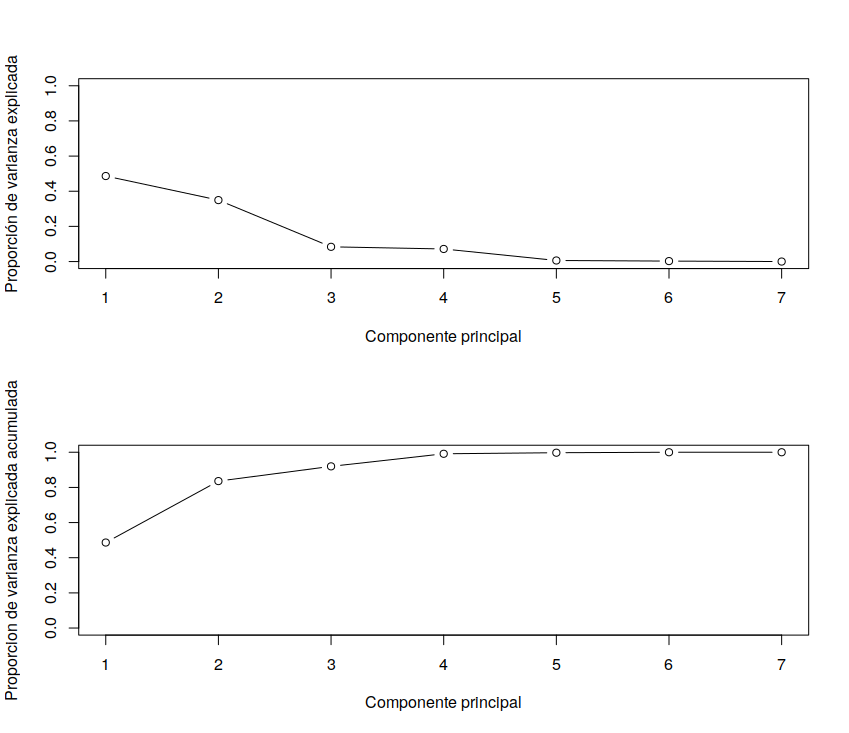
\includegraphics[scale=.35]{images/varPCA.png} 
	\label{i_var_PCA}
	\caption{Varianza explicada por las componentes principales}
\end{figure}
\end{frame}


\begin{frame}
\begin{figure}[h]
\centering
	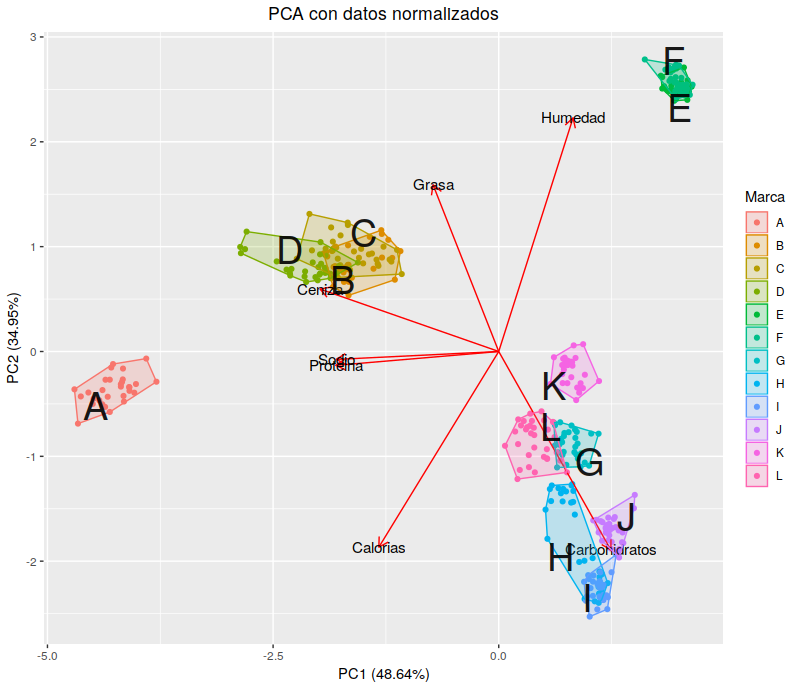
\includegraphics[scale=.35]{images/biplotPCA.png} 
	\label{i_biplot_PCA}
	\caption{Biplot PCA}
\end{figure}

\end{frame}

\begin{frame}{titulo}
\end{frame}

\begin{frame}{titulo}
\end{frame}

\end{document}